\documentclass[conference]{IEEEtran}
\usepackage{algorithm}
\usepackage{algpseudocode}
\usepackage{amsmath}
\usepackage{graphicx}

\newcommand{\BigO}[1]{\ensuremath{\operatorname{O}\left(#1\right)}}

\title{An Autonomous Meeting Assistant}
\author{951926 \and 1001231 \and 1024072 \and 1028907}
\date{\today}

\begin{document}
\maketitle

\begin{abstract}
  In this report, we present a system which performs the 1996 AAAI Mobile Robotics Competition task ``Call a meeting''\cite{AAAIcomp}. The robot was tasked with bringing a certain number of people to a meeting room previously determined as available. To complete the task, we use probabilistic road mapping, Monte Carlo localisation and a face detection module using the ROS framework, running on a Pioneer 3-DX platform modified with a tripod-mounted Kinect.
\end{abstract}
\section{Introduction}
Solutions to complex tasks often require the use of multiple techniques to solve different sub-problems, and this task is no exception. We were required to implement a localisation algorithm to determine the position of the robot, a probabilistic road map to allow paths to be planned through the space, a navigation algorithm for path planning, a method of exploring the space, and some way of detecting people. We then had to implement a system which would combine all of these separate modules into a single system that would complete the task. In the next section we present some background information about techniques that are often used to solve these sorts of problems. We then provide a detailed description of our system and evaluate its performance. Finally, we discuss the experimental results and suggest areas for improvement.
\section{Background}
\textbf{BRIEF INTRODUCTION TO SECTION NEEDED}

\subsection{Localisation}
The aim of localisation is to obtain an estimate of the position of a mobile robot using sensor data \cite{localisation}. While it is possible to use odometry data to do so, this data is inherently noisy and prone to error. In particular, odometry errors can arise from changes in the surface being traversed and the robot's weight, among others. An important point to note is that localisation can be performed with a prepared map, or generating a map in real-time. The much more complex latter problem is called simultaneous localisation and mapping, which we will not discuss here. See \cite{slam} for an introduction to the SLAM problem.

\subsubsection{Bayes Filter}
Many advanced localisation techniques are based on the Bayes filter, which uses a belief distribution $bel(x_t)$ to represent the state $x_t$. The calculation of $bel(x_t)$ at time $t$ is dependent on $bel(x_{t-1})$ at time $t-1$, the last action $u_t$, and the last measurement $z_t$. In the first step, called the prediction step, the prior belief $\overline{bel}(x_t)$ is calculated. This step merges two probability distributions; the prior belief over the previous state $x_{t-1}$, and the probability of transitioning from that state to the posterior state $x_t$ given that the action $u_t$ was taken. This step does not take into account any measurement taken in the posterior state, predicting based solely on the knowledge of the action taken. In the second step, the measurement update, the posterior belief is calculated by multiplying the prior belief with the probability of being in the posterior state given that the measurement $z_t$ was observed. The result of this multiplication is generally not a probability, and therefore requires normalisation using some constant $\alpha$. As there are usually multiple posterior states, $x_t$ is usually a state vector rather than a single state, and so the two steps will be applied multiple times in order to update the belief for each state being considered. The filter is recursive, requiring some idea of the initial belief $bel(x_0)$ at time $t=0$. The initial belief is either a distribution centred on $x_0$, in the case where the initial position is known, or a uniform distribution over the space otherwise.
\begin{algorithm}
  \caption{Bayes filter \cite{thrun}}
  \label{alg:bayesfilter}
  \begin{algorithmic}[1]
        \State \textbf{Algorithm Bayes\_filter}\textnormal{($bel(x_{t-1}), u_t, z_t$)}
        \For{\textnormal{all} $x_t$}
        \State $\overline{bel}(x_t)=\int P(x_t\mid u_t, x_{t-1})bel(x_{t-1})dx_{t-1}$
        \State $bel(x_t)=\alpha P(x_t \mid z_t)\overline{bel}(x_t)$
        \EndFor
        \State \Return $bel(x_t)$
  \end{algorithmic}
\end{algorithm}
As the Bayes filter is not restricted to finite state spaces, it is not possible to implement it for anything other than very simple problems. There are two families of algorithms for localisation, known as \emph{recursive state estimators}, with various properties that permit the use of the Bayes filter in more complex estimation tasks \cite{thrun}.
\subsubsection{Gaussian Filters}
The basic principle of the family of Gaussian filters is the use of multivariate normal distributions, which can be formulated from a mean $\mu$ and covariance $\Sigma$, to represent belief. As a result, the assumption that the system is a linear Gaussian system is made; the initial belief must be a Gaussian, and both the state transition function and measurement probability must be linear functions. Although Gaussian filters can be extended to non-linear systems, they perform best when the system meets the assumptions made. One of the main advantages of such filters is the computational complexity, which is polynomial with respect to the dimensionality of the state space. The main disadvantage is that Gaussians are unimodal and therefore cannot represent situations in which there are multiple hypotheses; a situation that is often encountered in robotics. Examples include the Kalman filter and the information filter, which are derived from two different ways of representing Gaussians. Both of these filters can be extended to non-linear systems by using a Taylor expansion to produce linear approximations of non-linear functions. Mixtures of Gaussians can also be used to extend the Kalman filter to encompass situations in which multiple hypotheses are required, but each extension increases the complexity of the algorithm. This extensibility is one of the reasons for the popularity of the Kalman filter in state estimation problems. With some extension, the information filter is particularly suited to multi-robot systems where information from multiple sources must be integrated, but issues with complexity have resulted in the Kalman filter becoming the more popular of the two for the majority of problems \cite{thrun}.
\subsubsection{Nonparametric Filters}
In contrast to Gaussian filters, nonparametric filters discretise the probability distribution and do not require assumptions of linearity and Gaussian belief distributions. Instead, the state is approximated by a finite number of values which are taken from the belief state at any given time. The number of these values can be varied, and nonparametric filters converge to the correct state as the number tends towards infinity. Because this family of filters does not impose restrictions on the posterior density, they are useful for problems such as global localisation, which require the state to be represented in a complex form. Global localisation is the problem of determining the position of the robot without knowing its initial position, resulting in global uncertainty and the need for a multimodal belief distribution. Although as a result nonparametric filters are more computationally expensive than Gaussian filters, it is possible to vary the number of values used to represent the belief to suit the problem using \emph{adaptive} techniques. Examples of these types of filters are the histogram and particle filters. The histogram filter decomposes a continuous space into some finite number of regions, each of which is assigned a probability based on the belief. Extensions include using dynamic decomposition techniques to use more coarse representations in regions with lower probability, and the use of \emph{selective updating}, which updates only the parts of the space which are deemed important. Particle filters approximate the belief by drawing a number of hypotheses called \emph{particles} randomly from the belief distribution. The most important part of the particle filter is the resampling step, which selects particles from the initial set proportional to an importance factor. This has the effect of concentrating particles in areas of high likelihood, reducing computational power spent in areas which are not relevant. Improving the sampling method and adapting the number of particles based on time and uncertainty lead to more effective and error-resistant particle filters. A property which is particularly useful to us is that particle filters are very easy to implement \cite{thrun}.

\begin{algorithm}
  \caption{Basic Monte Carlo Localisation \cite{thrun}}
  \label{alg:basicMCL}
  \begin{algorithmic}[1]
    \State \textbf{Algorithm MCL}\textnormal{($\mathcal{X}_{t-1}, u_t, z_t, map$)}
    \State $\bar{\mathcal{X}}_t=\mathcal{X}_t=\emptyset$
    \For{$m=1$ to $M$}
    \State $x_t^{[m]}=\textbf{sample\_motion\_model}(u_t,x_{t-1}^{[m]})$
    \State $w_t^{[m]}=\textbf{sensor\_model}(z_t,x_t^{[m]},map)$
    \State $\bar{\mathcal{X}}_t=\bar{\mathcal{X}}_t+\langle x_t^{[m]},w_t^{[m]}\rangle$
    \EndFor
    \For{$m=1$ to $M$}
    \State \textnormal{draw $i$ with probability $\propto w_t^{[m]}$}
    \State \textnormal{add $x_t^{[i]}$ to $\mathcal{X}_t$}
    \EndFor
    \State \textbf{return} $\mathcal{X}_t$
  \end{algorithmic}
\end{algorithm}

\subsubsection{The Markov Assumption}
One of the reasons that these filters are so efficient stems from the assumption that the Markov property holds. While this may not actually be the case, the Bayes filter that forms the base of these filters is robust to the violation of some of the requirements of the property. The Markov property states that the future states of the system do not depend on past states. In other words, considering all previous states of the system provides no additional information for predicting future states; all prediction can be done using only the current state. Previous states do not have to be included in calculations, and as a result do not need to be stored, which leads to faster computation and lower storage space requirements.

\subsubsection{Sensor \& Motion Models}
To actually use any of these filters to solve a localisation problem, it is necessary to model the sensors and motion of the robot. These models include some parameters representing the uncertainty attached to performing a specific action or receiving a certain measurement from a sensor. The motion model is used in the prediction step to determine the state transition probability $P(x_t\mid x_{t-1}, u_t)$; the probability of going from state $x_{t-1}$ to $x_t$ given that the action $u_t$ was performed. The sensor model is used to calculate $P(z_t\mid x_t,map)$, which represents the likelihood of the measurement $z_t$ being received in the state $x_t$ on a given map. The model incorporates knowledge about the noise parameters of the operating environment and the sensor being used in the form of probability densities. For example, a range sensor might include densities for correct measurements, measurements of unexpected obstacles, sensor failures and random measurements \cite{thrun}. 

Integrating the sensor and motion models into the particle filter results in an algorithm known as Monte Carlo localisation (MCL). The most basic version of MCL is shown in Algorithm \ref{alg:basicMCL}, in which $\mathcal{X}_{t-1}$ represents the particles from the previous time step, $M$ the total number of particles, $x_t^{[m]}$ the state of the $m$th particle with the action $u_t$ applied to it via the motion model, $w_t^{[m]}$ the importance weight of the $m$th particle, and $\bar{\mathcal{X}}_t$ the resampled set of particles. We use an adaptive implementation of MCL provided by the ROS system.

\subsection{Route Planning}
\subsubsection{Probabilistic Roadmaps}
A probabilistic roadmap (PRM) is a  multi-query motion planning algorithm for robots in static workspaces \cite{prm} which solves the problem of determining a path between start and goal configurations while avoiding collisions with obstacles in the workspace. The roadmap algorithm consists of two phases; the learning phase and the query phase.

In the first step of the learning phase, the construction step, a graph $G$ with vertices $V$ and edges $E$ is constructed. Free configurations are repeatedly sampled from the workspace and added to $V$. A free configuration is one where the robot does not intersect with walls or other obstacles in the workspace. Once a specified number of configurations have been sampled, the vertices in $V$ are connected. Attempts to connect two vertices $v$ and $n$ are only made if they are within a neighbourhood specified by a maximum distance $D$, and a connection is only made if the path between the two nodes is also valid, i.e. there is no configuration on the path where the robot intersects with walls or obstacles. If a connection is made, the edge from $v$ to $n$ is added to $E$. The second step of the learning phase is the expansion step, which is intended to improve the connectivity of the graph. This step can be skipped if a sampling algorithm which takes into account difficult (narrow) areas of the workspace is used in the construction step.
\begin{algorithm}
  \caption{Probabilistic Road Map Generation}
  \label{alg:prm}
  \begin{algorithmic}[1]
    \State \textbf{Algorithm generate\_PRM}\textnormal{($map$)}
    \State $V \leftarrow $\textbf{ sample\_vertices}\textnormal{($map$)}
    \For{$v\in V$}
    \State $a \leftarrow 0$
    % a is number of attempts, A is max attempts
    \While{$a<A \wedge \textbf{nconns} (v)<C$}
    \State $n \leftarrow$\textbf{ get\_closest}\textnormal{($V, v$)}
    \If{\textbf{dist}$(v,n)<D$}
    \If{$\neg\textbf{neighbour}(v,n)\wedge\textbf{vpath}(map,v,n)$}
    \State $E \leftarrow$\textbf{ connect}\textnormal{($v, n$)}
    \EndIf
    \ElsIf{$\neg \textbf{connected}(v,n) \wedge \textbf{vpath}(map,v,n)$}
    \State $E \leftarrow$\textbf{ connect}\textnormal{($v, n$)}
    \EndIf
    \State $a \leftarrow a + 1$
    \EndWhile
    \EndFor
  \end{algorithmic}
\end{algorithm}
Once the graph has been constructed, the query phase is entered. In this phase, the roadmap is used to find paths between start and goal configurations $s$ and $g$. In order to do this, $s$ and $g$ must first be connected to the graph using the same connection strategy used in the construction step. A graph search algorithm such as A* can then be used to find the shortest path between the two newly added vertices.

There are a number of ways in which the basic PRM algorithm can be improved. Most of these relate to the construction of the graph, as the graph is the part of the algorithm which most influences subsequent performance---if vertex placement is bad, then even if the graph search algorithm is good, it is possible that a path will not be found. The sampling method is particularly important, and many different techniques have been proposed to improve the coverage of the PRM. Roughly speaking, the techniques can be separated into uniform and advanced techniques. Uniform techniques include random sampling, sampling points on a grid, and splitting the workspace into cells and sampling some number of points from each of those subspaces. Uniform methods provide a simple but effective way of sampling, but may experience a drop in performance for more difficult workspaces, for example those with narrow corridors. In these cases, using advanced techniques such as medial axis sampling, which generates points at the midpoints between obstacles, can be effective \cite{sampling}. The strategy used to connect vertices can also affect the structure of the graph, which in turn affects the query phase. Improvements to the query phase can be made by using different graph search algorithms, but unless the graph is extremely dense the query time is negligible. Path smoothing can also be used on the path found by the graph search algorithm to improve it further; our version is found in Algorithm \ref{alg:pathsmooth}. In some cases, a path may not be found with the graph being used, and although expensive, re-generating the graph can sometimes remedy this problem.

\subsubsection{Rapidly Exploring Random Trees}
An RRT is a randomised data structure and algorithm that is also used to solve path planning problems. RRTs are designed to handle nonholonomic constraints and high degrees of freedom \cite{rrt}. Instead of sampling points and then attempting to connect them as in PRMs, RRTs are biased towards moving into unexplored areas of the state space by sampling points and being ``pulled'' towards them \cite{rrtprog}. There are several planners for RRTs, including a bidirectional planner where the tree grows from the start and goal vertices and uses an aggressive heuristic to connect the trees. In contrast to the multi-query PRM, an RRT is a single query algorithm; it is rerun every time a query is made. The properties of RRTs make them particularly suited to problems involving robot arms and robots with nonholonomic kinematics. As our platform can be considered holonomic, we mention RRTs for completeness.
\begin{algorithm}
  \caption{Path Smoothing}
  \label{alg:pathsmooth}
  \begin{algorithmic}[1]
    \State \textbf{Algorithm smooth\_path}\textnormal{($P, I, map$)}
    \For {$i = 0$ \textbf{to} $I$}
    \For {$j = 0$ \textbf{to} $\left|P\right|-2$}
    \State $a \gets P_i$
    \State $b \gets P_{i+1}$
    \State $c \gets P_{i+2}$
    \If{\textbf{vpath}$(map,a,c$)}
    \State \textbf{remove}($P,b$)
    \EndIf
    \EndFor
    \EndFor
    \State \textbf{return}\textnormal{ $P$}
  \end{algorithmic}
\end{algorithm}
\subsection{Exploration}
The problem of exploration revolves around taking actions to maximise information gain, given your current knowledge of the world. What is meant by information gain depends on the problem being solved. In many cases this is discovering the locations of walls and obstacles, but can also extend to more complex objectives such as determining the locations of specific objects, rooms, or people. The most basic form of exploration is the random walk, which ensures that any finite sequence of actions will be executed eventually \cite{thrunexploration}. ``Eventually'' is not good enough, however, and many improved exploration techniques have been proposed. Greedy techniques move the robot from its current location to the closest location that has not yet been explored \cite{greedy}. Frontier-based exploration moves to boundaries between open space and uncharted territory in order to gain the most possible new information \cite{frontier}. Distributed approaches using coordinated multi-robot systems have become an active area of research, and novel techniques drawing on economics concepts have been proposed \cite{multiexp, marketexp}. As with many solutions using distributed computing, the use of multiple ``processors'' allows the task to be completed in a shorter time, but requires the implementation of algorithms that can make good use of these increased capabilities.
\subsection{Robot Vision}
\section{Design}
\textbf{BRIEF INTRODUCTION TO SECTION NEEDED}
\subsection{Hardware \& Software}

\subsubsection{Robot Operating System}
The Robot Operating System (ROS) is an open source software framework developed by Willow Garage and the robotics community that provides libraries and tools for use in robot applications. The system comes with a series of \emph{stacks}; user contributed packages which can be used to perform SLAM, localisation and various other tasks that the user may not want to implement themselves, which means that development can be focused on solving the problem at hand. ROS code can be written in a variety of languages, including C++, Python and Java, and can be run on a large number of platforms, with support for humanoid robots, arms, quadrotors and many mobile robots.

The system uses a graph structure and uses data streams for communication between nodes, and as a result is robust to node failures. The use of data streams for communication allows for a high degree of modularity---a node written for one task can be used for another task with little or no modification required. Each node can have an arbitrary number of \emph{publishers} for sending messages to \emph{topics} and \emph{subscribers} for receiving them. One of the major strengths of the system is that when a message is sent, it does not have to be sent to a specific node; once it is published, the message is available to any node which is subscribed to that topic. All of the activity of the system is monitored by a master node which provides information about the state of the whole system, including node status and the currently active topics.

\subsubsection{Robotics Platform}
For the task, we were required to use a Pioneer 3-DX fitted with a Hokuyo URG-04LX laser rangefinder. The Pioneer is 455cm long, 381cm wide and 237cm high, and weighs 9kg, making it a relatively compact platform. It is fitted with six forwards-mounted and two side-mounted sonar sensors. The robot is powered by three batteries which provide a run time of 8-10 hours, assuming no accessories are attached. The robot is equipped with a differential drive system which has a 0cm turn radius, making it essentially holonomic. The maximum translation and rotation speeds are 1.2m/s and 300$^\circ$/s respectively \cite{pioneer}. 

The Hokuyo laser \cite{hokuyo}.

The Microsoft Kinect \cite{kinect}.

\subsection{System Structure}
Our implementation attempts to make the most of this system structure, with separate nodes for each subsystem. The actions of the system are controlled by the control node which is based on a finite state automaton. This node then hands off to other nodes when tasks need to be executed. The navigation node uses data from the localisation and PRM nodes to move between points in the map. Vision processing is done in a node written in C++ for speed, and the resulting data is used by the control node to make decisions about which actions to take.

\textbf{MENTION ALGORITHM COMPLEXITY?}
talk about implementation specifics - what algorithms we used, the sampling methods, localisation methods etc.
\subsubsection{Localisation Node}
We independently developed two localisation nodes which implemented augmented Monte Carlo localisation (AMCL), but which were not sufficiently error free that we were confident in using them for the combined task. Instead, we made the decision to use the ROS implementation of AMCL which comes with the software installation. By using a tried and tested implementation, we reduce the likelihood of bugs causing problems with the localisation. This is very important, as to move safely through the space it is necessary to have an accurate position estimate. \textbf{do we need justification here?}We had to tweak some parameters in the algorithm that we deemed necessary in the testing of our own algorithms while running in tandem with some of the other nodes that were to make up the final system. The AMCL defaults for filter updates are 0.2 metres for translation and 0.52 radians for rotation. We decreased both of these to 0.1 metres and 0.1 radians respectively in order to receive filter updates more often. A comparison of the performance of AMCL algorithms can be found in Figure \ref{fig:local}.
\subsubsection{PRM Node}
\begin{itemize}
\item map inflation
\item sampling method
\item connection strategy
\item path flattening
\end{itemize}
\subsubsection{Navigation Node}
\subsubsection{Vision Node}
\subsubsection{Control Node}
\section{Experimentation}
\textbf{BRIEF INTRODUCTION TO SECTION NEEDED}
\subsection{MCL Tracking Error}
\subsubsection{Aim}
The aim of this experiment is to compare the tracking error of three different MCL implementations; the built in ROS AMCL and two of our own implementations.
\subsubsection{Method}
As each MCL implementation has many different variables, we will use the set of variables that resulted in the best performance in past experiments. To provide accurate results, we require a ground truth, which will be obtained from the Stage simulator. We will run the experiment three times for each implementation and record the tracking error every second while the robot moves, until it reaches the end of its path. The tracking error is defined as the Euclidean distance between the ground truth and the estimated pose provided by the localisation at each point at which a measurement is taken. The robot will start from the same initial position and follow the same path, seen in Figure \ref{fig:locpath}, in each experiment.
\subsubsection{Results}
Figure \ref{fig:local} shows the tracking errors for each implementation, with error bars representing the standard deviation over three runs. Apart from two anomalous points at 13 and 25 seconds at which all implementations experience an increase in tracking error, the deviation of AMCL is significantly lower than the other two implementations. The average deviation over the three runs for AMCL is 0.019m, compared to averages of 0.071m and 0.085m for Penny and Leslie respectively. It is clear that to obtain accurate position estimates we should make use of ROS AMCL.

\begin{figure}
  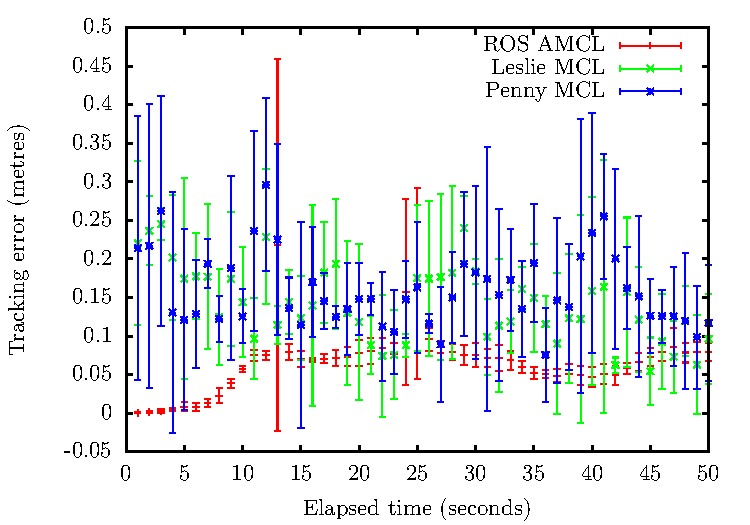
\includegraphics[width=\columnwidth]{tracking_stdev}
  \caption{Comparison of Tracking error of ROS AMCL and two independently developed AMCL algorithms}
  \label{fig:local}
\end{figure}
\begin{figure}
  \caption{Path used for tracking error experiment.}
  \label{fig:locpath}
\end{figure}
\subsection{PRM}
inflated map - show inflated map superimposed onto the original map
Redo experiment for sampling methods. short, medium, long path length. Display image of map with one of the routes displayed and show the difference between the sampling methods. Find the optimum route by sampling a massive number of vertices on to the space and then finding a route using that---the flattened path is then the most optimal route, and we compare the other routes to this route for each experiment.

Redid sampling experiments - now have comparison for neighbourhood, threshold and nearestN strategies on 4 different paths, including trying to get into the corridor. 5,10,20,30 maxconn for each strategy, inflation radius of 5 so that you can just about get into the corridor. random vertices:25,50,100,200,400,800, grid step 0.5,1,2,4, cell size 1,2,4,6, target per cell 2,5

\textbf{REDO THIS ONCE THE ABOVE DATA IS COMPILED}Best sampling: (approximate) optimum path found for each path by using grid sampling with a step of 0.2m and 50 max connections and neighbourhood connection strategy. Screenshots available in screenshots dir. Repeated experiments five times for cell and random, once only for grid. 5,10,20,30 maxconnections. Used results from previous experiments on the sampling strategy, but compared the best parameters for each. Also checked whether the corridor which causes issues was accessible when using each strategy as a measure of its ability to populate tight spaces. Not necessarily a good evaluation, since grid may be good on this map by accident, but terrible on others. new\_prmlogs contains data.


\subsection{Vision}
\subsection{Exploration}
Coverage experiments info: cell and grid done for cell size and grid spacing of 10,8,6,4,2,1, with cell repeated three times for each. The fov max distance was 3.5, angle 57, minimum distance 0.3. Started at 2.80,18.97,40 in stage. Max move speed 0.7m/s, max rotation speed 0.4 rad/sec. Ran until the end of the exploration path was reached.
\subsection{Whole System !RENAME THIS!}
\section{Discussion}
\subsection{Performance}
\subsection{Potential Improvements}
the path generated to do exploration could be improved by using heuristic techniques. multiple robots
\subsection{Conclusions}
\bibliographystyle{ieeetr}
\bibliography{report}
\end{document}
